\documentclass[border=3pt,tikz]{standalone}
% Shared look for every TikZ figure in these notes.
% Included by each standalone figure file; also keeps the figures consistent
% with the colours used in the PDF and on the website.

\usepackage{tikz}
\usepackage{pgfplots}
\pgfplotsset{compat=1.18}
\usetikzlibrary{arrows.meta, decorations.markings, decorations.pathmorphing,
                patterns, calc, positioning}
\usepackage{amsmath}

% Series colours are the three validated categorical slots also used by the
% interactive widgets, so a path drawn in the printed notes and the same path on
% the website are the same colour. They clear the colour-vision-deficiency and
% contrast checks as a set; every path is direct-labelled as well, so colour is
% never the only thing carrying identity.
\definecolor{duPurple}{HTML}{68246D}
\definecolor{duBlue}{HTML}{2A78D6}
\definecolor{duRed}{HTML}{EB6834}
\definecolor{duGreen}{HTML}{1BAF7A}
\definecolor{duGrey}{HTML}{4D4D4D}

\tikzset{
  % heavier default lines and arrow tips, so diagrams stay clear when zoomed
  every picture/.append style = {line width=0.7pt, >={Stealth[length=3mm]}},
  axisline/.style   = {-{Stealth[length=3.4mm]}, line width=1.0pt, black},
  path1/.style      = {duBlue,   line width=1.6pt},
  path2/.style      = {duRed,    line width=1.6pt},
  path3/.style      = {duGreen,  line width=1.6pt},
  statedot/.style   = {circle, fill=black, inner sep=1.8pt},
  arrowhead/.style  = {decoration={markings,
                        mark=at position #1 with {\arrow{Stealth[length=3.4mm]}}},
                       postaction={decorate}},
  lbl/.style        = {font=\normalsize},
  slbl/.style       = {font=\small, duGrey},
  workfill/.style   = {duPurple, opacity=0.16},
}

% larger labels in plots as well
\pgfplotsset{every axis/.append style={label style={font=\normalsize}, tick label style={font=\small}, line width=0.9pt}}

% Jet engine and dam spillway (textbook photos) with the control volumes drawn
% on the board, next to the textbook open-system sketch. Overlay coordinates
% are in pixels of each photo, measured from its top-left corner.
\begin{document}
\begin{tikzpicture}[
    cv/.style={duRed, dashed, line width=1.3pt, preaction={draw=white, solid, line width=2.4pt}},
    flow/.style={-{Stealth[length=2.8mm]}, duRed, line width=1.4pt,
                 preaction={draw=white, line width=3pt, -}}]
  % jet engine: 288 x 162 px
  \node[anchor=north west, inner sep=0] (jet) at (0,0)
    {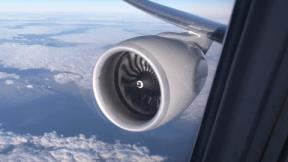
\includegraphics[width=4.4cm]{../img/ch4-open-systems-jet-clean.png}};
  \begin{scope}[shift={(jet.north west)}, x=4.4cm/288, y=-4.4cm/288]
    \draw[cv] plot[smooth cycle, tension=0.7] coordinates
      {(122,43) (165,33) (206,31) (215,56) (212,98) (188,113) (134,121) (101,101) (98,68)};
    \draw[flow] (22,106) .. controls (50,104) and (65,100) .. (86,91);
    \draw[flow] (196,46) .. controls (215,40) and (230,30) .. (250,20);
  \end{scope}
  % dam spillway: 291 x 164 px
  \node[anchor=north west, inner sep=0] (dam) at (5.2,0)
    {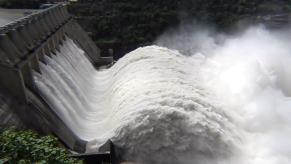
\includegraphics[width=4.4cm]{../img/ch4-open-systems-dam-clean.png}};
  \begin{scope}[shift={(dam.north west)}, x=4.4cm/291, y=-4.4cm/291]
    \draw[cv] plot[smooth cycle, tension=0.6] coordinates
      {(66,44) (94,62) (101,90) (95,118) (72,115) (39,91) (48,68)};
  \end{scope}
  % open system: heat, work and mass cross the boundary (textbook sketch)
  \node[anchor=west, inner sep=0] at (10.4,-1.24)
    {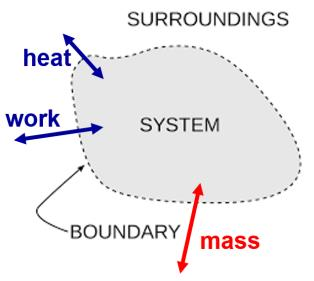
\includegraphics[width=4.2cm]{../img/ch4-open-systems-system-clean.png}};
\end{tikzpicture}
\end{document}
